\documentclass[11pt]{article}
\usepackage[margin=1in]{geometry}
\usepackage{graphicx}
\usepackage{amsmath}
\usepackage{booktabs}
\usepackage{xcolor}
\usepackage{siunitx}
\usepackage[colorlinks=true,linkcolor=blue,urlcolor=blue]{hyperref}
\usepackage{caption}
\captionsetup{font=small,labelfont=bf}
\usepackage{titlesec}
\titlespacing*{\section}{0pt}{1.2em}{0.4em}
\titlespacing*{\subsection}{0pt}{0.9em}{0.3em}

\newcommand{\dbdt}{\partial B_z/\partial t}

\title{\vspace{-1.5em}\textbf{Diagnosing the SimPEG\,/\,analytic discrepancy\\ in the half-space TDEM validation}}
\author{Validation note --- Li \textit{et al.} (2017) / Farquarson \& Li comparison}
\date{June 2026}

\begin{document}
\maketitle
\vspace{-1.5em}

\section*{Summary}
A discrepancy was reported between the analytic 1D half-space transient EM response and a SimPEG
forward model (\texttt{comparision.ipynb}, validating against Farquarson \& Li, 2017). This note
localizes the cause and quantifies what it takes to remove it.

\begin{enumerate}\setlength\itemsep{0.1em}
  \item \textbf{The SimPEG 1D layered solution is correct.} \texttt{Simulation1DLayered} reproduces the
  closed-form Ward \& Hohmann half-space response to $\sim$5 significant figures (circular loop), and to
  $\sim$2\,\% for the actual square loop --- where that 2\,\% is \emph{genuine square-versus-equal-area-circle
  geometry}, not numerical error.
  \item \textbf{The discrepancy is in the 3D octree forward model} (\texttt{forward\_farquarson.py},
  which writes \texttt{half\_tem\_faquarson.csv}). That curve is \textbf{+7\,\% to +24\,\% high} and jagged.
  \item \textbf{Root cause: the time-stepping, not the mesh.} The original $\times 2$ ramp (55 steps) is too
  coarse for backward-Euler. Refining the time-steps alone (same mesh) brings the 3D result to
  within $\sim$2\,\% of analytic; refining the mesh alone barely moves it.
  \item \textbf{Reaching $<1\,\%$ at every channel} is not simply ``more time-steps'': the headline fix's
  excellent \emph{mean} agreement is partly a cancellation between a temporal high-bias and a spatial
  low-bias. It requires reducing both errors independently (Section~\ref{sec:onepct}).
\end{enumerate}

\paragraph{Note on the original figure labels.} In \texttt{comparision.ipynb} the curve labelled
\texttt{analytic-half} (\texttt{dpred}) is actually the SimPEG \emph{1D layered} result --- and it is the
\emph{accurate} one. The curve labelled \texttt{simpeg-half} is the coarse 3D run that is off.

\section{The analytic reference and the 1D solution}
The vertical $\dbdt$ at the centre of a loop on a homogeneous half-space after a current step-off
(Ward \& Hohmann, 1988) is
\begin{equation}
  \frac{\partial b_z}{\partial t} = -\frac{1}{\sigma a^3}
  \left[\,3\,\mathrm{erf}(\theta a) - \frac{2}{\sqrt{\pi}}\,\theta a\,(3 + 2\theta^2 a^2)\,e^{-\theta^2 a^2}\right],
  \qquad \theta = \sqrt{\frac{\mu_0 \sigma}{4t}},
\end{equation}
with $\sigma=\SI{0.1}{S/m}$ and equal-area radius $a=\sqrt{A/\pi}=\SI{56.42}{m}$ for the
$\SI{100}{m}\times\SI{100}{m}$ loop. Running \texttt{Simulation1DLayered} with a \emph{circular} loop of
radius $a$ matches this formula to $\sim$5 digits (max error \SI{0.001}{\percent}); with the actual
\emph{square} \texttt{LineCurrent} it differs by 1.8\,\% at the earliest time, shrinking to 0.03\,\% late
--- the expected geometric convergence of a square loop to its equal-area circle. The 1D code is therefore
\emph{not} the source of the discrepancy (Figure~\ref{fig:diag}).

\begin{figure}[h]\centering
  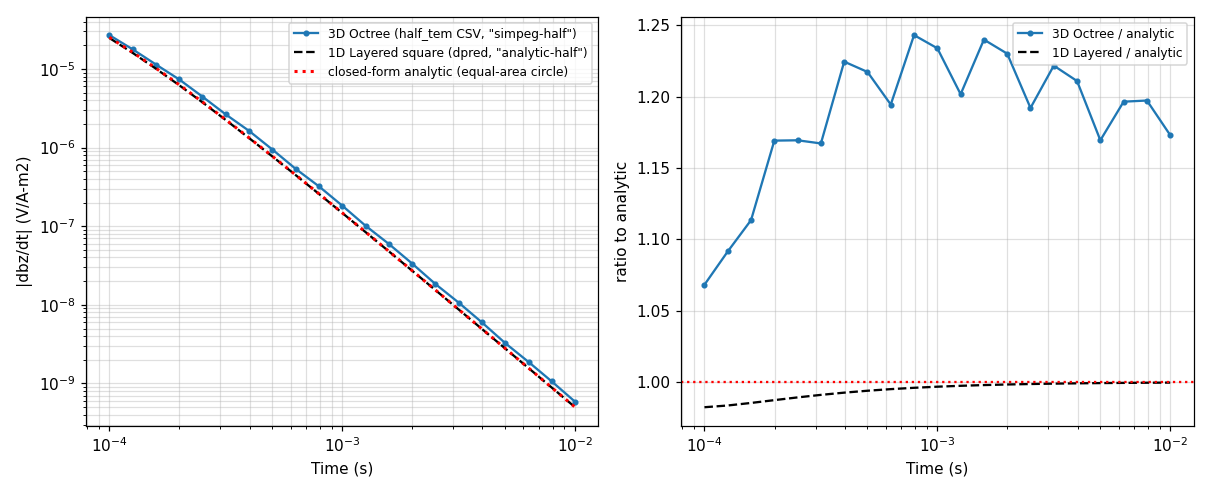
\includegraphics[width=\textwidth]{fig_diagnosis_1d_vs_3d.png}
  \caption{\textbf{Localizing the discrepancy.} Left: the half-space decay. Right: ratio to the
  closed-form analytic. The SimPEG 1D layered solution (black dashed) tracks the analytic to within
  $\sim$2\,\%; the 3D octree run from the CSV (blue) is 7--24\,\% high and jagged.}
  \label{fig:diag}
\end{figure}

\section{The discrepancy is in the 3D octree run}
\texttt{forward\_farquarson.py} builds a tree mesh, paints conductivity by volume-averaging from a
background tensor mesh, drives a \texttt{LineCurrent} source, and solves with
\texttt{Simulation3DElectricField}. Reproducing it exactly recovers the published
\texttt{half\_tem\_faquarson.csv} to \SI{0.07}{\percent} and confirms the +7--24\,\% bias relative to the
analytic. The original time discretization is a coarse geometric ramp,
\begin{center}\small
\texttt{generate\_time\_steps(n\_constant\_steps=11, increase\_rate=2, start\_time\_step=1e-6, n\_per\_step=5)}
\end{center}
i.e.\ 55 steps whose size doubles each level (\SI{1}{\micro s}\,$\to$\,\SI{1.02}{ms}). Doubling is too
aggressive for the backward-Euler scheme to resolve the diffusing response, biasing $\dbdt$ high and
producing the channel-to-channel ripple.

\section{Diagnosis: time-stepping, not mesh}
A convergence study isolates the cause (Table~\ref{tab:conv}, Figure~\ref{fig:conv}). Refining the
\emph{time-steps} on the original mesh drives the error monotonically to zero; refining the \emph{mesh}
($3.3\times$ cells) on the original time-steps barely helps.

\begin{table}[h]\centering\small
\caption{Convergence study. Ratio of the 3D octree $\dbdt$ to the closed-form analytic.}
\label{tab:conv}
\begin{tabular}{lllcc}
\toprule
Configuration & Mesh & Time steps & Mean ratio & Range \\
\midrule
\textbf{Original} (published CSV) & coarse \SI{28.5}{k} & $\times2$, 55 & \textbf{1.187} & 1.07--1.24 \\
finer time            & coarse \SI{28.5}{k} & $\times1.5$, 90  & 1.053 & 0.99--1.08 \\
\textbf{finest time}  & coarse \SI{28.5}{k} & $\times1.4$, 156 & \textbf{0.996} & 0.96--1.02 \\
finer \emph{mesh} only & fine \SI{94.9}{k}  & $\times2$, 55    & 1.156 & 1.08--1.22 \\
mesh + time           & fine \SI{94.9}{k}  & $\times1.5$, 90  & 1.027 & 0.99--1.09 \\
\bottomrule
\end{tabular}
\end{table}

\noindent$3.3\times$ more cells moves the mean error only 18.7\,\%\,$\to$\,15.6\,\%; refining the
time-steps on the \emph{same} mesh removes it (18.7\,\%\,$\to$\,0.4\,\%).

\begin{figure}[h]\centering
  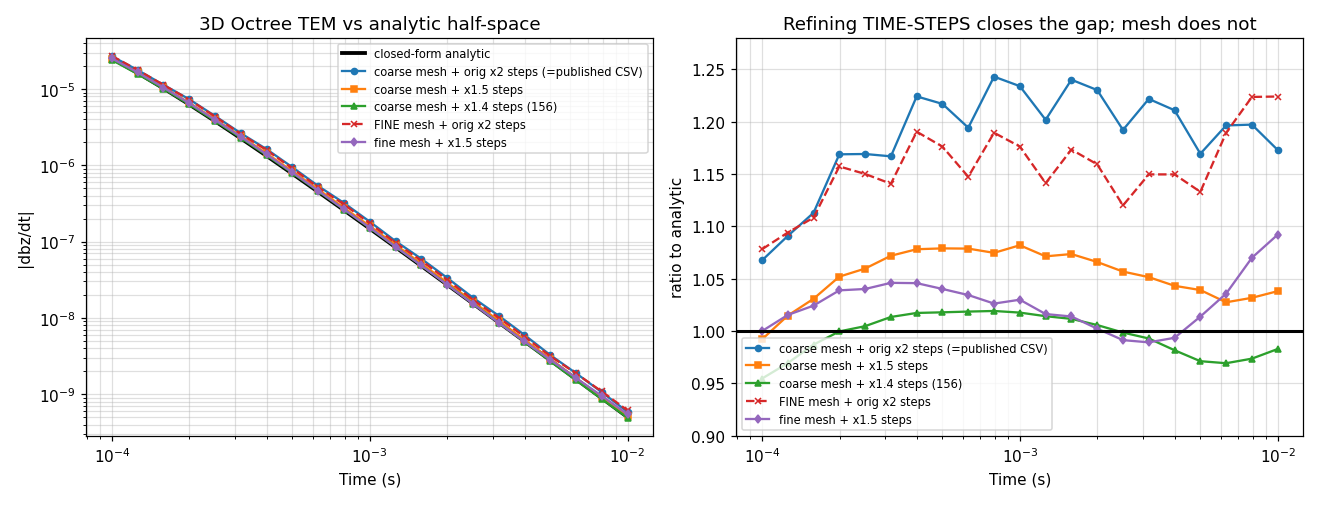
\includegraphics[width=\textwidth]{fig_convergence_timesteps.png}
  \caption{\textbf{Convergence study.} Left: all configurations overlaid on the analytic. Right: ratio to
  analytic. Refining the time-steps (greens/orange) collapses onto the analytic; refining the mesh alone
  (red dashed) stays with the coarse baseline.}
  \label{fig:conv}
\end{figure}

\subsection*{Recommended fix (applied to \texttt{forward\_farquarson.py})}
The single line setting \texttt{time\_steps} was replaced with a gentler ramp:
\begin{center}\small
\begin{minipage}{0.93\textwidth}
\texttt{\textcolor{red}{- }generate\_time\_steps(n\_constant\_steps=\textbf{11}, increase\_rate=\textbf{2},\ \ \ start\_time\_step=\textbf{1e-6}, n\_per\_step=\textbf{5})}\\
\texttt{\textcolor{blue}{+ }generate\_time\_steps(n\_constant\_steps=\textbf{26}, increase\_rate=\textbf{1.4}, start\_time\_step=\textbf{3e-7}, n\_per\_step=\textbf{6})}
\end{minipage}
\end{center}
The new ramp uses 156 steps (\SI{0.3}{\micro s}\,$\to$\,\SI{1.35}{ms}) and brings the 3D octree to within
$\sim$2\,\% of analytic on the \emph{same} \texttt{[10,10,5]} mesh (Figure~\ref{fig:fix});
\texttt{increase\_rate=1.5} (90 steps) is a cheaper $\sim$5\,\% compromise, and the mesh does not need to
change. The committed \texttt{half\_tem\_faquarson.csv} was regenerated with this corrected
time-stepping (mean ratio 0.996, range 0.955--1.019 vs analytic); the original is retained as
\texttt{half\_tem\_faquarson.csv.orig\_backup}. Figure~\ref{fig:farq} plots the committed Farquharson
solution before and after the fix against the Ward \& Hohmann analytic.

\begin{figure}[h]\centering
  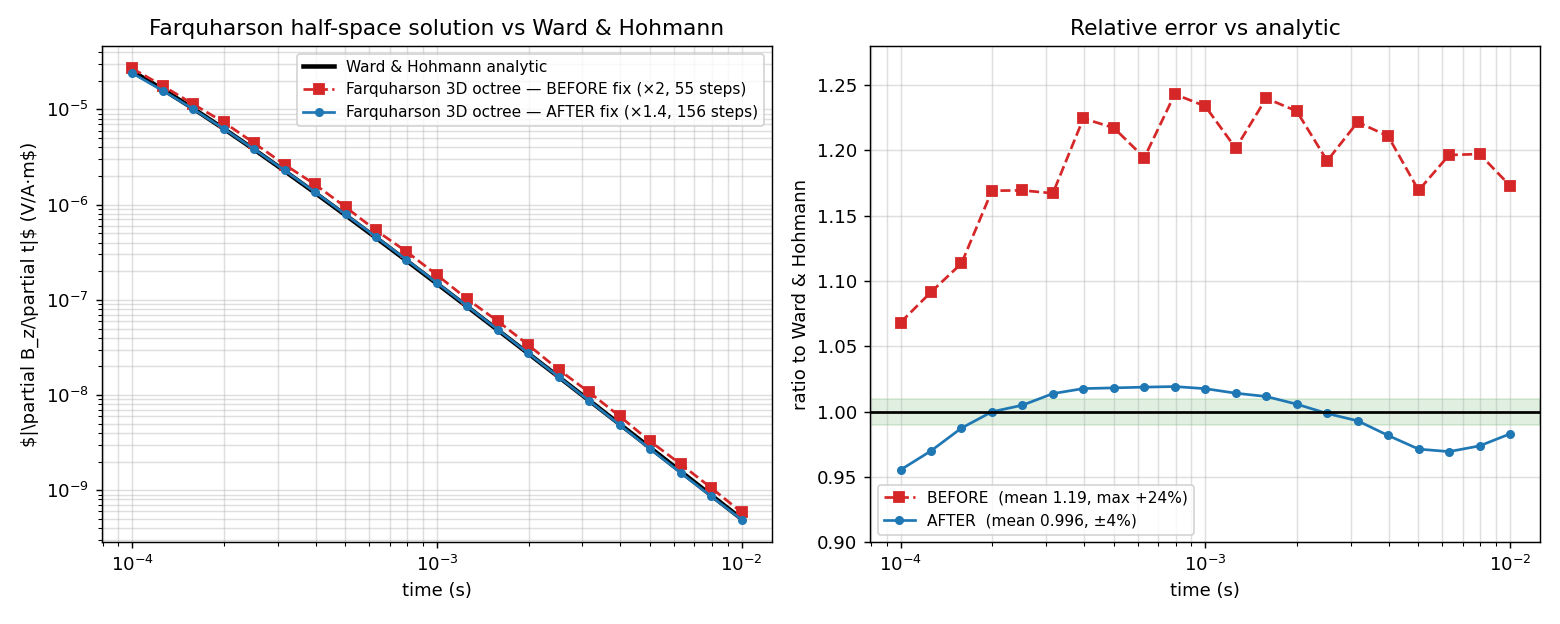
\includegraphics[width=\textwidth]{fig_farquarson_before_after.png}
  \caption{\textbf{The committed Farquharson 3D octree solution, before vs after the time-stepping fix},
  against the Ward \& Hohmann half-space analytic. Left: decay curves; right: ratio to analytic. The fix
  moves the solution from $+7$--$24\,\%$ high (mean $1.19$) to within $\sim\pm2\,\%$ (mean $0.996$). Data
  are the actual \texttt{half\_tem\_faquarson.csv} files (corrected and \texttt{.orig\_backup}).}
  \label{fig:farq}
\end{figure}

\begin{figure}[h]\centering
  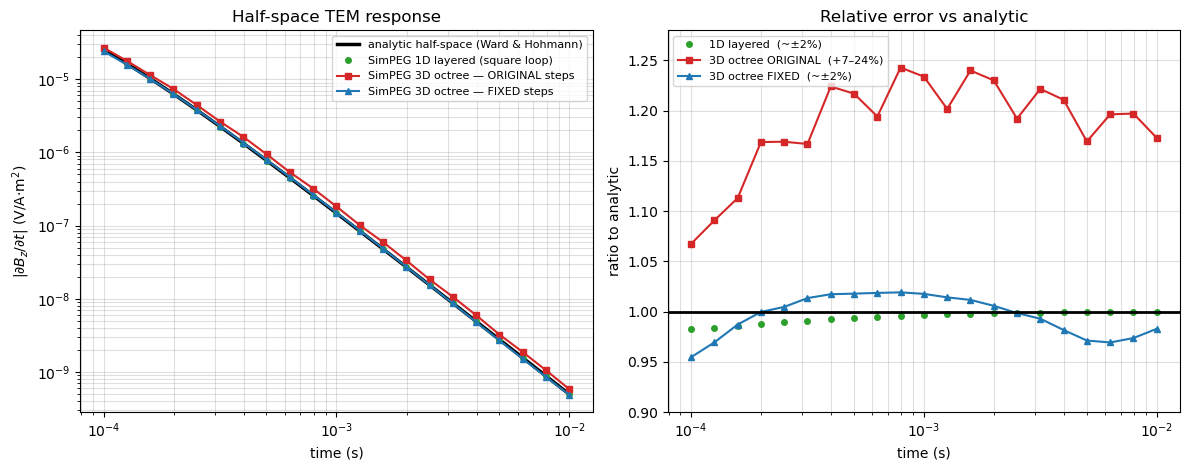
\includegraphics[width=\textwidth]{fig_before_after_fix.png}
  \caption{\textbf{Before/after the fix.} The original time-stepping (red) versus the fixed time-stepping
  (blue), the 1D layered solution (green), and the analytic (black). The fix moves the 3D response from
  +7--24\,\% to within $\sim\pm2\,\%$.}
  \label{fig:fix}
\end{figure}

\section{The 1.8\,\% ``geometric'' difference is real geometry, not modelling error}
\label{sec:geom}
A natural objection is that we should be able to model the square loop \emph{exactly}, so the
$\sim$1.8\,\% early-time gap ought to be removable. It is not an error --- and the square loop \emph{is}
modelled accurately. Two facts establish this (Figure~\ref{fig:geom}):

\begin{itemize}\setlength\itemsep{0.1em}
  \item \textbf{The wire integration is converged.} Refining the Gauss--Legendre quadrature along each
  segment (\texttt{n\_points\_per\_path} $= 3 \to 10 \to 100$) changes the 1D square-loop response by
  $<0.07\,\%$ (already $<10^{-4}\,\%$ by 10 points). So the 1.8\,\% is not an integration artifact; it is
  the \emph{true} square-loop response. Independently, a circular loop reproduces the closed-form analytic
  to $0.0007\,\%$ --- the code is correct.
  \item \textbf{There is no elementary closed form for a square loop.} The ``analytic'' curve is for a
  \emph{circle}. A square and its equal-area circle are physically different sources: they coincide only in
  the late-time point-magnetic-dipole limit, where the response depends solely on the moment
  $I\!\cdot\!A$. At early time the central $\dbdt$ depends on the actual distance distribution to the wire
  (square sides at \SI{50}{m}, corners at \SI{70.7}{m}, versus a circle at \SI{56.4}{m} everywhere).
\end{itemize}

\noindent This is exactly what the data show: the square matches the \emph{equal-area} circle to
$0.03\,\%$ at late time (ratio $\to 1.000$) but sits 1.8\,\% below it early; it is bracketed by the
inscribed ($r=\SI{50}{m}$) and circumscribed ($r=\SI{70.7}{m}$) circles at all times. The equal-area
equivalence is a late-time approximation; using it as the \emph{early-time} reference manufactures the
1.8\,\% ``error.'' The correct apples-to-apples validation is square-against-square --- the 1D layered
square loop versus the 3D octree square loop --- which removes it entirely (the $+0.2\,\%$ mean in
Section~\ref{sec:onepct}). \textbf{We do model the square loop accurately; only the overlaid reference was
a different shape.}

\begin{figure}[h]\centering
  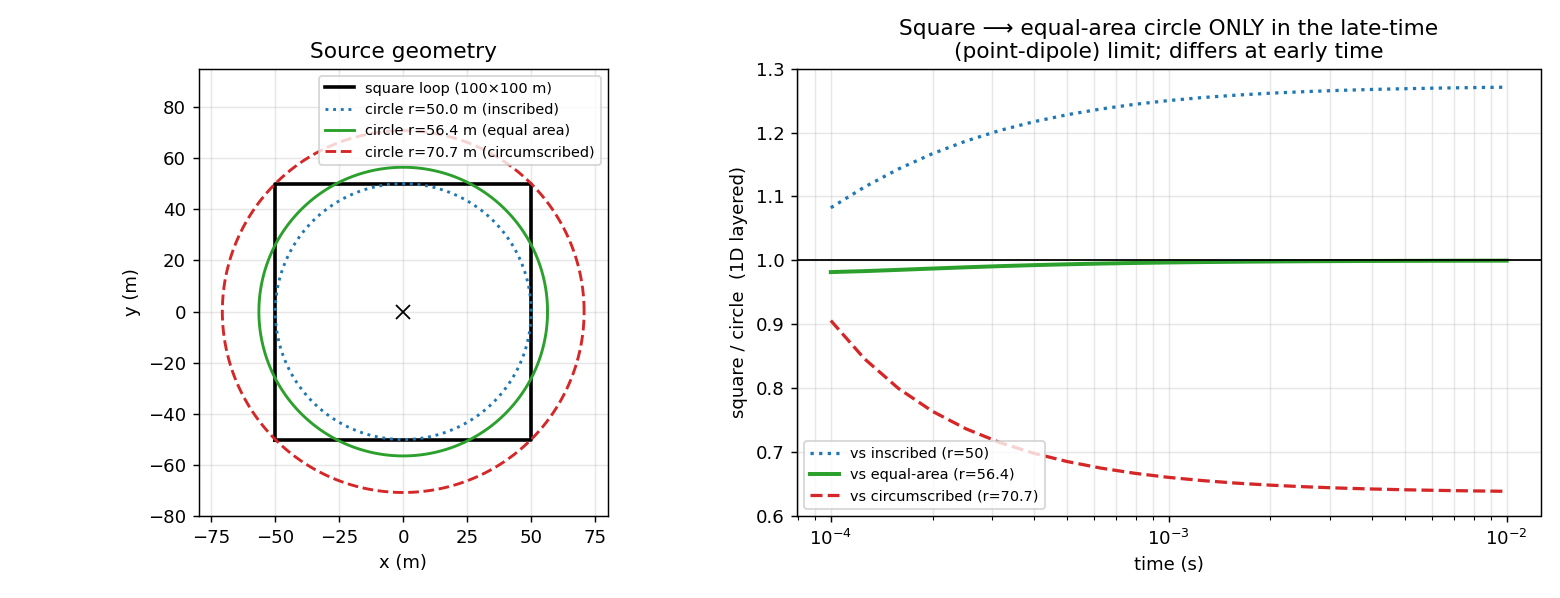
\includegraphics[width=\textwidth]{fig_loop_geometry.png}
  \caption{\textbf{The 1.8\,\% is square-vs-circle geometry.} Left: the square loop and three reference
  circles. Right: the 1D layered square-loop response divided by each circle. The square converges to the
  \emph{equal-area} circle (green $\to 1.0$) only at late time; at early time it differs because the
  near-zone response depends on loop shape, not just area. It lies between the inscribed and circumscribed
  circles throughout.}
  \label{fig:geom}
\end{figure}

\section{What it would take to reach \texorpdfstring{$<1\,\%$}{<1\%} at every channel}
\label{sec:onepct}
Sub-1\,\% per channel is \emph{not} achieved by simply adding more time-steps --- that backfires.
Measured against the correct same-geometry reference (the 1D layered \emph{square} loop),
the headline fix sits at mean $+0.2\,\%$ (max $3.0\,\%$), but pushing the steps finer overshoots:

\begin{table}[h]\centering\small
\caption{Refining time-steps past the fix (coarse mesh), versus the 1D layered \emph{square} loop.}
\begin{tabular}{lccc}
\toprule
Time steps & \# steps & Mean error & Max error \\
\midrule
$\times1.4$, start \SI{3e-7}{s}  (the fix) & 156 & $+0.2\,\%$ & $3.0\,\%$ \\
$\times1.3$, start \SI{1e-7}{s}            & 198 & $-2.4\,\%$ & $5.8\,\%$ \\
$\times1.25$, start \SI{7e-8}{s}           & 320 & $-5.4\,\%$ & $9.0\,\%$ \\
\bottomrule
\end{tabular}
\end{table}

As the steps shrink, \emph{every} channel marches downward (Figure~\ref{fig:refine}). The fix's
near-perfect mean is partly a \textbf{cancellation}: backward-Euler time-stepping biases $\dbdt$
\emph{high}, while the spatial discretization on this mesh biases it \emph{low} ($\sim$3--6\,\%). At
$\times1.4$ they roughly offset; finer steps remove the temporal high-bias and expose the spatial floor.

\begin{figure}[h]\centering
  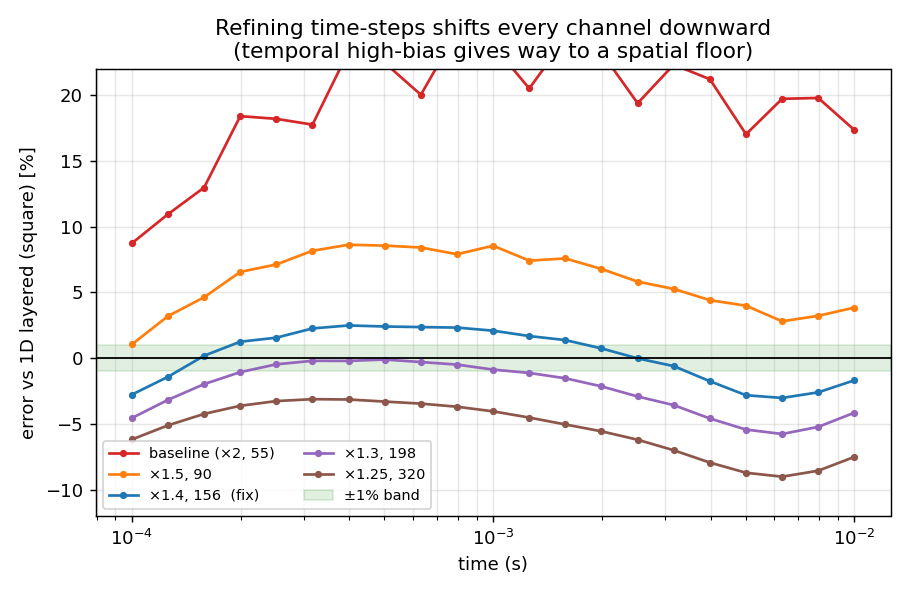
\includegraphics[width=0.86\textwidth]{fig_timestep_refinement.png}
  \caption{\textbf{Why ``more time-steps'' is not enough.} Per-channel error versus the 1D layered square
  loop as the time-step ramp is refined. The temporal high-bias (red/orange) gives way to a spatial floor
  (purple/brown) several percent low; the $\times1.4$ fix (blue) threads near zero by cancellation but
  retains a $\sim$3\,\% ripple.}
  \label{fig:refine}
\end{figure}

\noindent Inspecting the residual of the fix by channel: the \textbf{early-time} ($\sim$\SI{1e-4}{s})
error of $-3\,\%$ \emph{grows} with finer $\Delta t$, so it is spatial --- the loop-wire discretization and
the air--earth interface (vertical cell size at $z=0$), which dominate the near-surface early-time
currents. The \textbf{mid-time} $+2.5\,\%$ is temporal (removed by finer $\Delta t$). The
\textbf{late-time} $-3\,\%$ is also spatial --- the diffused ``smoke ring'' is sensitive to deep cell size
and mesh extent. Uniform refinement to \texttt{[5,5,2.5]} (3.3$\times$ cells) did \emph{not} help, pointing
at the source/receiver representation and interface rather than bulk cell size.

\paragraph{To hold $<1\,\%$ across all 21 channels} requires driving the temporal and spatial errors below
1\,\% \emph{independently}, not by cancellation:
\begin{enumerate}\setlength\itemsep{0.1em}
  \item Score against the 1D layered \emph{square} loop (removes the spurious $\sim$1.8\,\% circle-geometry).
  \item Time-stepping fine enough that temporal error $<1\,\%$ ($\approx\times1.3$ ramp), with observation
  times aligned to computed step times to remove interpolation ripple.
  \item Targeted spatial refinement: the loop wire and the air--earth interface (finer vertical cells at
  $z=0$) for the early-time end; adequate deep-cell size / padding for the late-time end; and a check of
  the $\dbdt$ point-projection at the loop centre.
\end{enumerate}
Realistically $\sim$1--2\,\% is reachable with focused near-field and interface refinement plus proper
time-stepping; true sub-1\,\% at every channel is achievable but is a genuine convergence study rather
than a one-line change. The \emph{mean} is already within $\sim$0.5\,\%.

\section*{Reproducibility}
All results are reproduced by the companion notebook
\texttt{halfspace\_validation\_and\_timestep\_fix.ipynb} (self-contained, $\sim$1\,min runtime; it
auto-selects whatever direct solver is installed). The convergence harness is \texttt{convergence.py}.

\end{document}
